The key measures for Study 2 were the case-count data (after our transformation) and the set of human predictions of the duration of the epidemic ($t_{predicted}$).  Figure \ref{fig:Study_2_Multi} shows the results.  In the left panel, we see the case-count data and the human predictions super-imposed, along with the polynomial fits.  The three vertical lines indicate the change points in the case-count data.  The first noticeable feature in this panel is the large region of time after the second change point for which the case-counts and the human prediction move in opposing directions.  Another interesting feature is that the case-count curve was much flatter prior to the second change point compared to after it.  The final point of interest in this panel the similar slope of the two time-series in terms shortly prior to and after the third change point.  The second panel, showing the first derivatives of the case-count polynomials, provides a more nuanced understanding of the relation between the human predictions and the case-counts.  The major features of this panel are as follows:  (i) the strongest and most sustained growth of the case-counts is the period for which we see the strongest and most sustained negative growth of the human predicted durations; (ii) during the period mentioned in (i) we don't see positive growth in the human prediction until the case-count growth starts to slow.  In short, from the derivatives, we see two clear relations.  First, when the case-count growth is strong, the human growth is negative.  Second, when the case-count growth is slow or lessening from a high growth period, the human predictions show growth. 

\begin{figure}
    \centering
    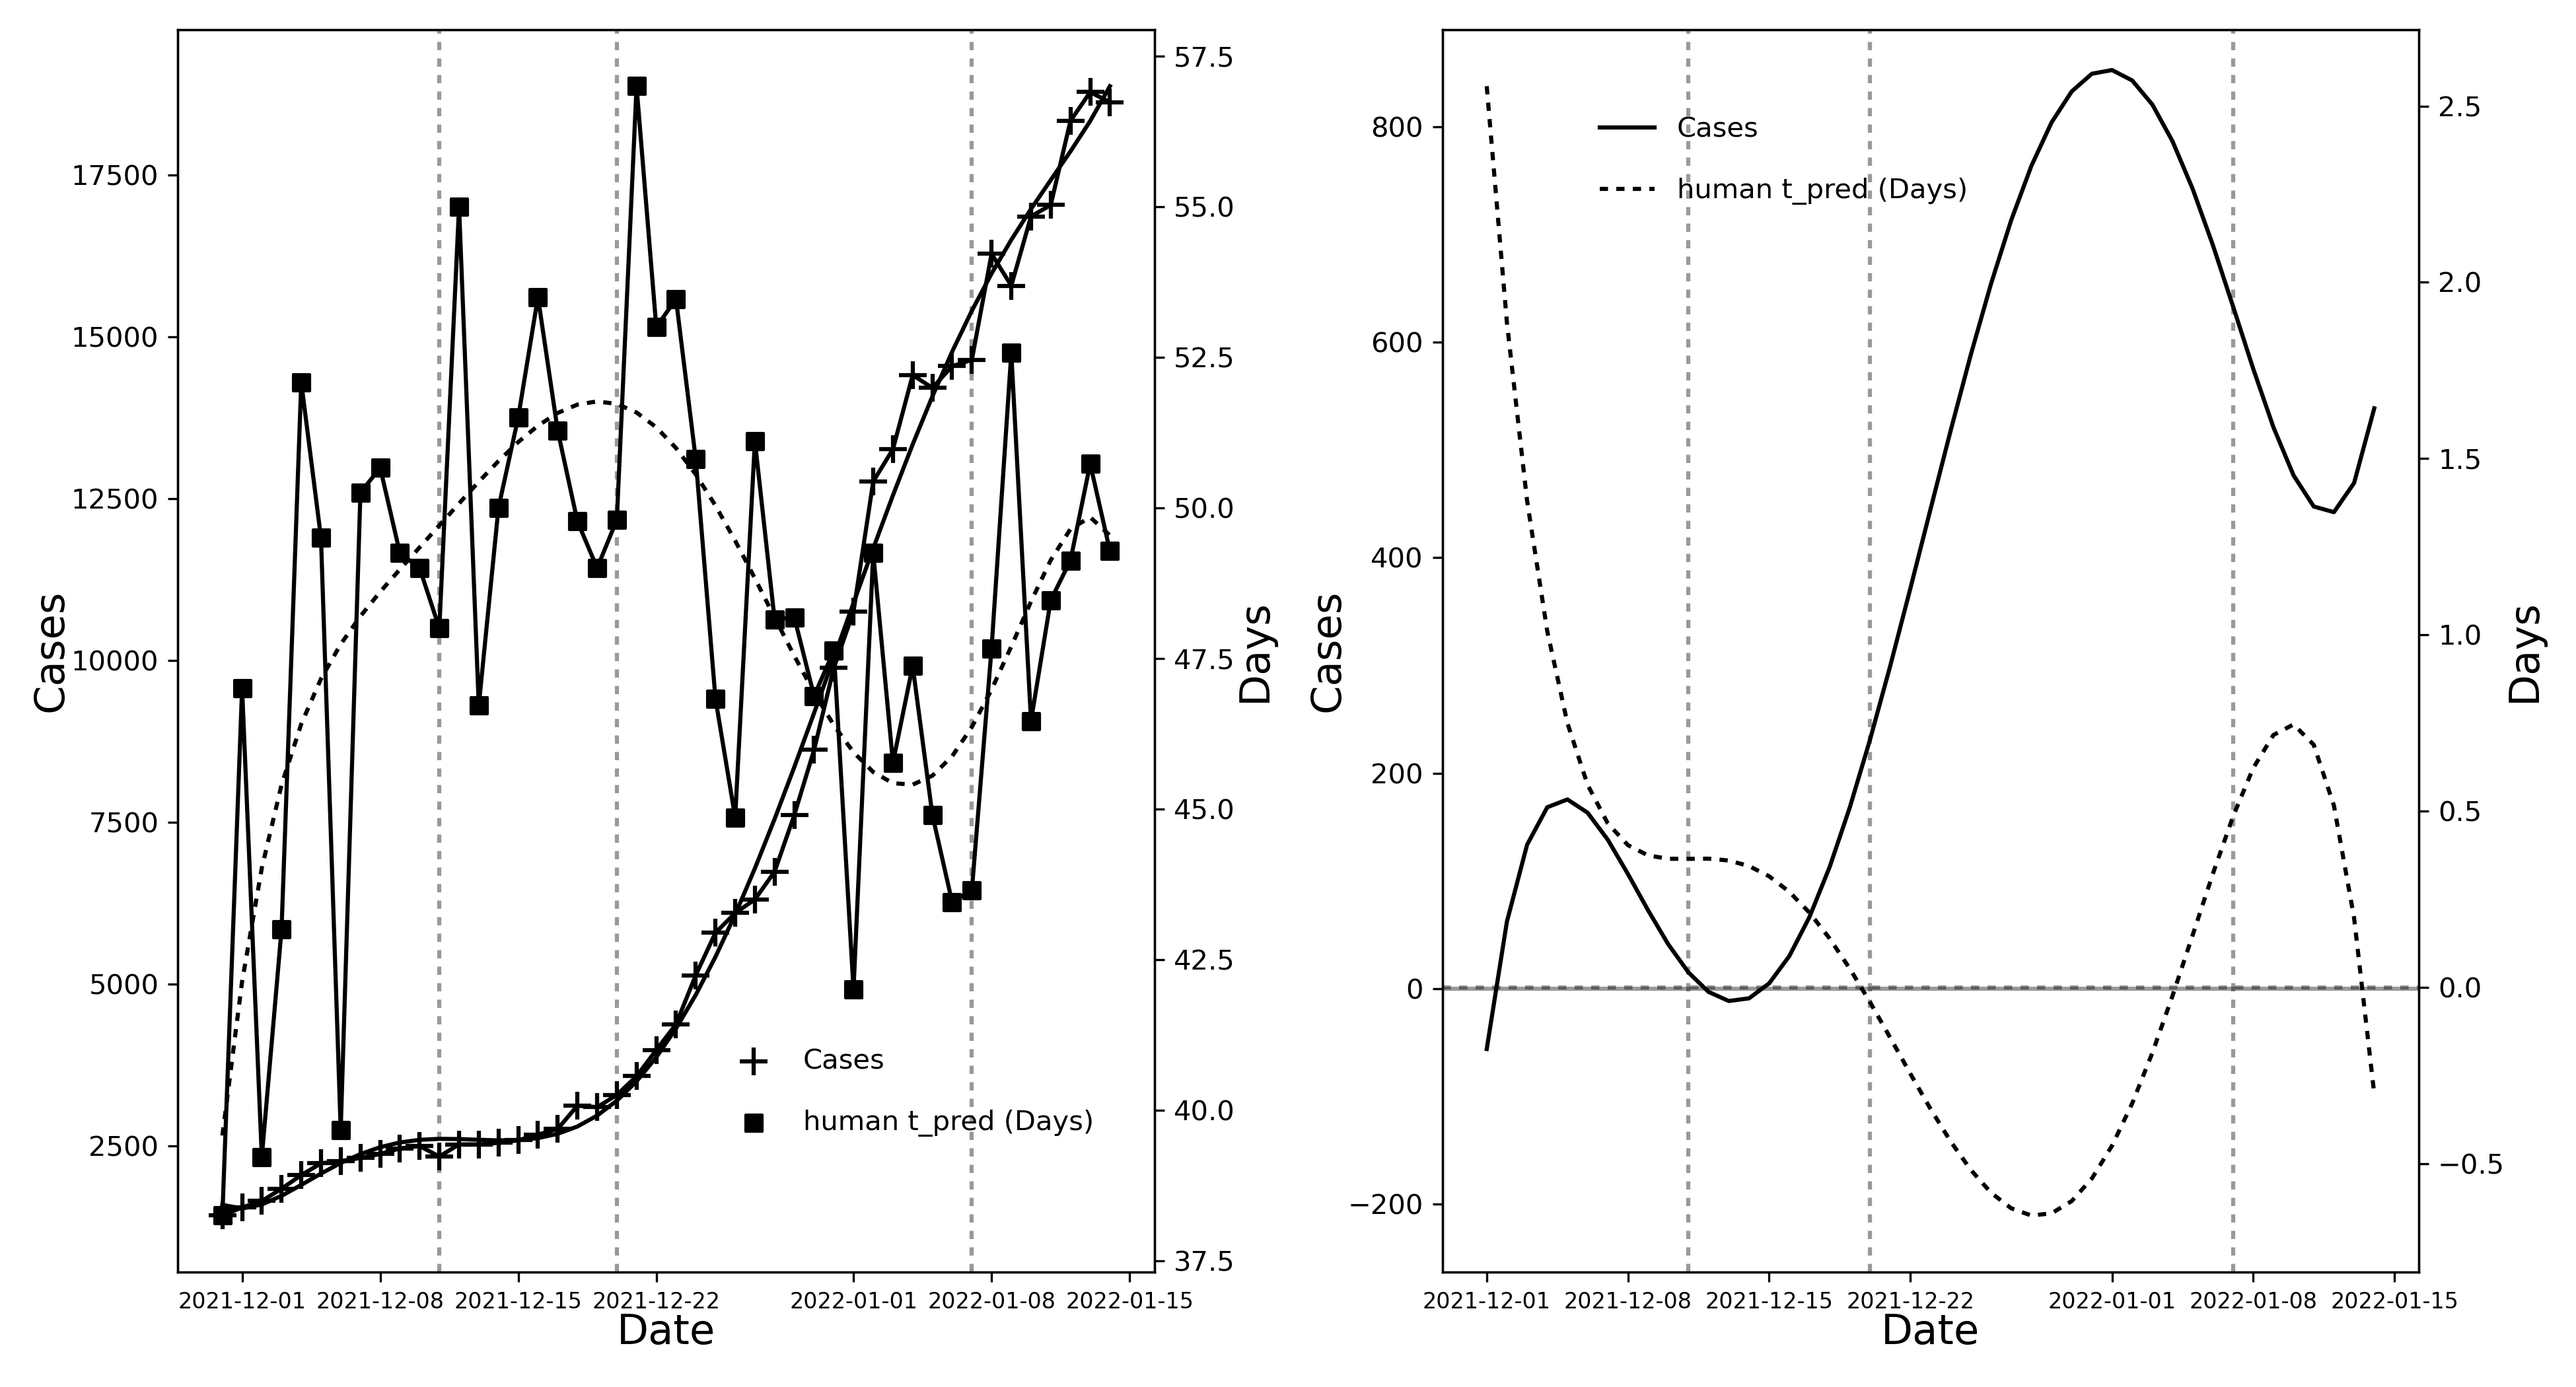
\includegraphics[width=\linewidth]{Figures/Study_2_Figure.png}
    \caption{The left panel illustrates the case-count data and the human predictions super-imposed, along with the polynomial fits.  The three vertical lines indicate the change points in the case-count data.  The right panel shows the first derivatives of the polynomials for the case-count and human predicted durations.}
    \label{fig:Study_2_Multi}
\end{figure}